\section{Branch and Bound method}
The Branch and Bound method uses a divide and conquer strategy to solve an ILP problem, exploring its set of feasible solutions.
Let $F$ be the set of a feasible solution to the problem:
\begin{align*}
    \min       \quad & c^T     \\
    \text{s.t} \quad & x \in F \\
\end{align*}
The method is split into two phases:
\begin{enumerate}
    \item \textit{Branch}, the problem is partitioned in simpler subproblems.
    \item \textit{Bound}, the subproblems are solved, and the optimal solution is found.
\end{enumerate}

The two phases are applied recursively until a solution is found;
if a problem is unsolvable in the bound phase, it is branched again until is simple enough to be solved.
This technique can be applied to a wide range of problems, not limited to ILP problems.

\paragraph*{Branching}
The set of solutions $F$ is partitioned in $k$ subsets:
\[ F = F_1 \cup,  \ldots,  \cup F_k \quad F_i \cap F_j = \emptyset \ \forall,  i \neq j \]
Let $z_i$ be:
\[ z_i = \min\left\{ c(x), \middle\vert\, x \in F_i \right\} \quad i = 1,,  \ldots,  , k \]
The solution $z$ is finally found as:
\[ z = \min\left\{ c(x), \middle\vert\, c \in F \right\} = \min\left\{ z_i,,  \ldots, , z_k \right\} \]

\paragraph*{Bounding}
For each subproblem $\min\left\{ c(x), \middle\vert\, x \in F_i \right\}$, whose solution is found in the partition of $F$, the optimal solution $z_i$ is found by either:
\begin{enumerate}
    \item Determining an optimal solution of $\min\left\{ c(x), \middle\vert\, x \in F_i \right\}$.
    \item Proving that $F_i = \emptyset$.
    \item Proving that $z_i \geq z$, where $z$ is the optimal solution of the original problem found so far.
\end{enumerate}
If the subproblem is not solved, it's mandatory to generate a new subproblem by branching it again.

\paragraph*{Generic Branch and Bound Method}
If the lower bound $b(F_i)$ of the optimal solution of the subproblem $\min\left\{ c(x), \middle\vert\, x \in F_i \right\}$ is greater than the optimal solution $z$ found so far, the subproblem is discarded, as it cannot contain a better solution than the one found so far.
At any point, the algorithm keeps in memory a set of active subproblems and the cost $U$ of the best feasible solution found so far;
initially, $U$ is either $\infty$ or the cost of the best feasible solution found by the heuristic method (if any).
A typical step of the algorithm is:
\begin{enumerate}
    \item Select an active subproblem $F_i$ to be solved
    \item If the subproblem is infeasible, delete it; otherwise, compute $b(F_i)$ for the corresponding subproblem
    \item If $b(F_i) \geq U$, delete $F_i$
    \item If $F_i$ is feasible and $b(F_i) < U$, either:
        \begin{itemize}
            \item obtain an optimal solution to the subproblem
            \item breaks the corresponding subproblem into further subproblems, which are added to the set of active subproblems.
        \end{itemize}
\end{enumerate}

There are several parameters that can be arbitrarily chosen;
there is not a fixed rule for many of them, as the best choice depends on the problem to be solved.

\begin{enumerate}
    \item There are multiple ways of choosing an active subproblem.
    \item There are multiple ways of breaking a subproblem into further subproblems.
    \item There are multiple ways of computing the lower bound $b(F_i)$.
\end{enumerate}

\subsubsection{Branching Tree}
The branching tree is a tree that represents the branching process of the ILP problem.
Each node of the tree represents a subproblem of the ILP problem, and each edge represents a branching step.
A branching tree may not contain all possible nodes or all possible leaves $2^d$;
a node of the tree has no child (is fathomed) if:
\begin{enumerate}
    \item The initial constraint and those on the arcs from the root to the node are infeasible.
    \item The optimal solution of the linear relaxation is an integer.
    \item The value $C^T \overline{x}_{\text{LP}}$ of the optimal solution $\overline{x}_{\text{LP}}$ of the linear relaxation is worse than the best feasible solution $z$ found so far.
\end{enumerate}
This criterion is called the branching criterion: it allows discarding a large number of nodes (subproblems) that would not lead to a valid solution, thus reducing the size of the tree.

\begin{figure}[H]
    \centering
    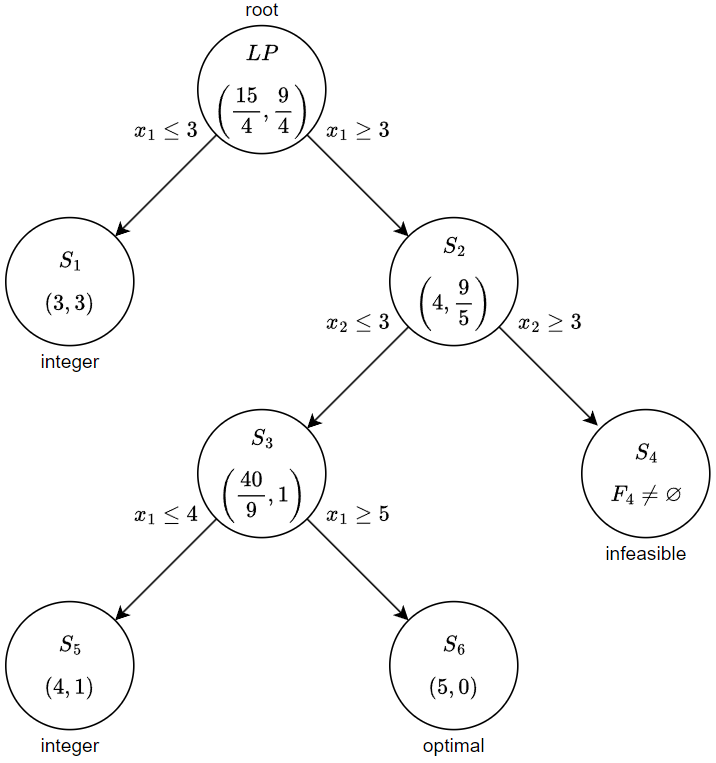
\includegraphics[width=0.25\linewidth]{images/ilp3.png}
    \caption{Branching tree}
\end{figure}

\subsubsection{Branch and Bound for the ILP problem}
Given an ILP problem:
\[ \min\left\{ c^T x, \mid\, Ax = b, \ x \in \mathbb{N} \right\} \]
the Branch and Bound method can be applied to find the optimal solution $z$.
\paragraph*{Branching}
Partition $F$ into subregions, let $\overline{x}$ denote an optimal solution of the linear relaxation of the ILP:
\[ \min\left\{ c^T x, \mid\, Ax = b, \ x \geq 0, \ x \in \mathbb{R} \right\} \quad z_{\text{LP}} = c^T \overline{x} \]
If $\overline{x}$ is integer, then it's also optimal for the ILP problem;
otherwise, the ILP is partitioned into two subproblems:
\begin{gather}
    \min\left\{ c^T x, \middle\vert\, Ax = b, x \leq \left\lfloor \overline{x} \right\rfloor \right\} \label{eq:branch1}\tag{ILP 1} \\
    \min\left\{ c^T x, \middle\vert\, Ax = b, x \geq \left\lceil \overline{x} \right\rceil \right\} \label{eq:branch2}\tag{ILP 2}
\end{gather}
where the symbols $ \left\lfloor \overline{x} \right\rfloor $ and $ \left\lceil \overline{x} \right\rceil $ denote the floor and ceiling of the vector $\overline{x}$.

Choosing the variable $x_h$ whose fractional value is closest to $0.5$, hoping to obtain two subproblems that are balanced is not always the best approach.
The best solution is the strong branching:
try to branch on some candidate variables (fractional basic ones) evaluating the corresponding objective function values and actually branch on the variable that yields the best improvement in the objective function value.

\paragraph*{Bounding}
Determine a lower or upper bound, if the ILP is respectively a minimization or a maximization problem on the optimal value $z_i$ of a subproblem of ILP by solving its linear relaxation.

In order to choose the node (subproblem) to be solved, the following criteria can be used:
\begin{itemize}
    \item \textit{Deeper nodes first} (depth-first search strategy): chooses the node with the greatest depth in the tree of subproblems
        \begin{itemize}
            \item simple to implement, easy to optimize
            \item may lead to a large tree of subproblems if the wrong branching variable is chosen
        \end{itemize}
    \item \textit{More promising nodes first} (best-bound first strategy): chooses the node with the best linear relaxation value $b(F_i)$
        \begin{itemize}
            \item generates a small tree of subproblems
            \item the subproblems are less constrained, leading to longer times to find a feasible solution and improve it
        \end{itemize}
\end{itemize}

\paragraph{Remarks on the Branch and Bound method}

\paragraph*{General remarks}
\begin{itemize}
    \item Branch and Bound is also applicable to mixed ILP problems: at the branch step, just consider that the fractional variables are integer and the integer variables are continuous
    \item Finding a good initial feasible solution with a heuristic algorithm may improve the method's performance by providing a better lower or upper bound for (respectively) maximization or minimization problems.
    \item Branch and Bound can also be used as a heuristic method for solving the ILP problem: the algorithm stops when the best feasible solution found so far is better than the best integer solution found so far.
\end{itemize}

\paragraph*{Efficient solution of the linear relaxation}
\begin{itemize}
    \item There's no need to solve the linear relaxations of the ILP subproblem from scratch at each branching step: the solution of the linear relaxation of the parent node can be used as a starting point for the solution of the linear relaxation of the child node.
    \item An optimal solution of the linear relaxation with a single additional constraint can be found via a single iteration of the Dual Simplex method (the simplex method applied to the dual problem) to the optimal Branch and Bound of the previous node (linear relaxation of the parent subproblem).
\end{itemize}

\paragraph*{Applicability of Branch and Bound approach}

The Branch and Bound method can be adapted to solve any discrete optimization problem and many non-linear optimization problems;
two procedures need to be changed:
\begin{itemize}
    \item The partition of the feasible region into subregions (branch).
    \item The determination of a bound on the optimal value of the subproblem (bound).
\end{itemize}

